\documentclass[tikz,border=12pt]{standalone}
% Shared visual language for standalone EMT block diagrams.
\usepackage{amsmath}
\usetikzlibrary{arrows.meta,backgrounds,calc,fit,positioning}

\tikzset{
    emt diagram/.style = {>={Stealth[length=2.4mm]}},
    line/.style        = {semithick, rounded corners=6pt},
    block/.style       = {draw, semithick, fill=white,
                          minimum height=1cm, minimum width=2.3cm},
    hblock/.style      = {block, minimum width=2.24cm, minimum height=1.3cm},
    vblock/.style      = {block, minimum width=1.3cm, minimum height=2.24cm},
    sum/.style         = {draw, semithick, fill=white, circle,
                          inner sep=2.6pt},
    signal/.style      = {circle, fill, inner sep=1.4pt,
                          label distance=3pt},
    sig/.style         = {font=\small},
    pm/.style          = {font=\scriptsize},
    wire jump/.style   = {line,
                          preaction={draw=white, line width=3pt,
                                     line cap=round}},
    enclosure/.style   = {draw, dashed, semithick, rounded corners=4pt},
    operator enclosure/.style = {enclosure, inner xsep=7mm, inner ysep=6mm}
}


\begin{document}
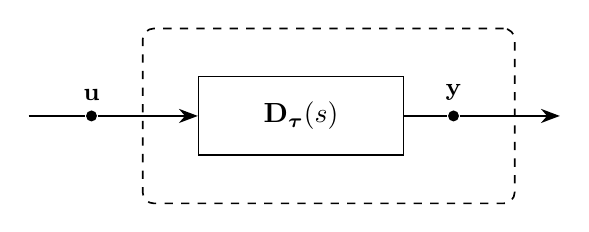
\begin{tikzpicture}[emt diagram]

\node[block, minimum width=2.6cm] (delay)
    {$\mathbf{D}_{\boldsymbol{\tau}}(s)$};

\node[signal, label={[sig]above:$\mathbf{u}$}] (uin)
    at ($(delay.west)+(-1.35,0)$) {};
\draw[line] ($(uin)+(-0.8,0)$) -- (uin);
\draw[->, line] (uin) -- (delay.west);

\node[signal, label={[sig]above:$\mathbf{y}$}, right=0.55cm of delay]
    (yout) {};
\draw[line] (delay.east) -- (yout);
\draw[->, line] (yout) -- ++(1.35,0);

\begin{scope}[on background layer]
    \node[operator enclosure, fit=(delay)(yout)] {};
\end{scope}

\end{tikzpicture}
\end{document}
